\documentclass[12pt]{article}
\usepackage{../lp,graphicx,amsmath}
\usepackage{tkz-berge}
% Cross-references for handout numbers.
\usepackage{amsfonts}
%\usepackage{amsthm}
\usepackage{hyperref}
\usepackage{amssymb}
%\usepackage[capitalize]{cleveref}
\usepackage{xcolor}

%\input{handouts}

\newcounter{chapnum}

\newtheorem{definition}{Definition}[chapnum]
\newtheorem{remark}{Remark}[chapnum]
\newtheorem{theorem}{Theorem}[chapnum]
\newtheorem{lemma}[theorem]{Lemma}
\newtheorem{corollary}[theorem]{Corollary}
\newtheorem{proposition}[theorem]{Proposition}
\newtheorem{claim}[theorem]{Claim}
\newtheorem{observation}{Observation}[chapnum]

\renewcommand{\thesection}{\arabic{chapnum}.\arabic{section}}
\renewcommand{\thefigure}{\arabic{chapnum}.\arabic{figure}}


\newenvironment{proof}{\noindent{\bf Proof:} \hspace*{1em}}{
        \hspace*{\fill} $\triangle$ }
\newenvironment{proof_of}[1]{\noindent {\bf Proof of #1:}
        \hspace*{1em} }{\hspace*{\fill} $\triangle$ }
\newenvironment{proof_claim}{\begin{quotation} \noindent}{
        \hspace*{\fill} $\diamond$ \end{quotation}}
\newenvironment{solution}{\noindent{\bf Solution:} \hspace*{1em}}{
        \hspace*{\fill} $\triangle$ }


\newcommand{\R}{{\mathbb R}}
\newcommand{\Z}{{\mathbb Z}}
\newcommand{\Q}{{\mathbb Q}}
\newcommand{\C}{{\mathbb C}}
\newcommand{\N}{{\mathbb N}}
\newcommand{\lin}{\operatorname{lin}}
\newcommand{\aff}{\operatorname{aff}}
\newcommand{\cone}{\operatorname{cone}}
\newcommand{\conv}{\operatorname{conv}}
\newcommand{\vol}{\operatorname{vol}}
\newcommand{\poly}{\operatorname{poly}}




\newcommand{\CF}[1]{{\color{purple}[CF: #1]}}


\newlength{\toppush}
\setlength{\toppush}{2\headheight}
\addtolength{\toppush}{\headsep}

\newcommand{\htitle}[2]{\noindent\vspace*{-\toppush}\newline\parbox{6.5in}
{Massachusetts Institute of Technology \hfill 18.453: Combinatorial Optimization 
\newline
\textbf{Instructor:} Cole Franks \quad \textbf{Notes: }Michel Goemans and Zeb Brady \hfill#2\newline
\mbox{}\hrulefill\mbox{}}\vspace*{1ex}\mbox{}\newline
\begin{center}{\Large\bf #1}\end{center}}

\newcommand{\handout}[2]{\thispagestyle{empty}
 \markboth{ #1 \hfil #2}{ #1 \hfil #2}
 \pagestyle{myheadings}\htitle{#1}{#2}}


\setlength{\oddsidemargin}{0pt}
\setlength{\evensidemargin}{0pt}
\setlength{\textwidth}{6.5in}
\setlength{\topmargin}{0in}
\setlength{\textheight}{8.5in}


\newcounter{exercisenum}
\newcounter{exercisetot}
\setcounter{exercisetot}{0}



\newenvironment{exercises}{
	\begin{list}{{\bf Exercise \arabic{chapnum}-\arabic{exercisenum}. \hspace*{0.5em}}}
	{\setlength{\leftmargin}{0em}
	 \setlength{\rightmargin}{0em}
	 \setlength{\labelwidth}{0em}
	 \setlength{\labelsep}{0em}
	\usecounter{exercisenum}
      \setcounter{exercisenum}{\theexercisetot}}}{\setcounter{exercisetot}{\theexercisenum}\end{list}}


\newenvironment{pseudocode}{
    \begin{list}{}{
        \renewcommand{\makelabel}{$\triangleright$}
        \setlength{\topsep}{0pt}
        \setlength{\leftmargin}{32pt}
        \setlength{\labelwidth}{14pt}
        \setlength{\labelsep}{0mm}
        \setlength{\itemindent}{0mm}
        \setlength{\itemsep}{-3pt}
        \setlength{\itemsep}{0mm}
        \setlength{\parsep}{0pt}%
        \setlength{\listparindent}{0pt}
    }
}
{
    \end{list}
}

\newcommand{\rank}{\operatorname{rank}}

\setlength{\topmargin}{-1in}
\setlength{\textheight}{9.7in}
%\usepackage{epsfig}
\begin{document}

%\handout{QUIZ 1}{April 11th, 2017}

\noindent {\Large 18.453 Final, Spring 2021} \\
~\\
Do not distribute.
\paragraph{Note: } Some people initially downloaded a final with slightly different wordings. The differences were very minor, but nonetheless I apologize for the mixup. This was, of course, taken into account during grading. These solutions are for the updated final.

%For best practice I suggest trying to complete it under these conditions. Afterwards please tell me if 2 hours felt like enough.
%Please write the solutions as neatly as possible and show your steps. Your grade will be the average of these two grades.


\begin{enumerate}
\item (5 points; 1 each) Answer true or false. If true, provide a concise reason (no rigor necessary) and if false, exhibit a counterexample or concise reason.
\begin{enumerate}
\item For every graph $G$, the \emph{undirected} incidence matrix $A_G$ of $G$ is totally unimodular. For instance, the path of length two $(\{1,2,3\}, \{(1,2), (2,3)\})$ has the undirected incidence matrix
$$ \begin{bmatrix}
1 & 1 & 0 \\
0 & 1 & 1
\end{bmatrix}. $$
\item Given two matroids $M_1 = (E, I_1)$, $M_2 = (E, I_2),$ the pair $(E, I_1 \cup I_2)$ is a matroid.
%\item Given two matroids $M_1 = (E, I_1)$, $M_2 = (E_, I_2),$ the pair $$(E, \{X \cup Y: X \in I_1, Y\in I_2\})$$ is a matroid.
%\item Suppose $A \in \R^{m\times n}, b \in \R^m$ and that $Ax \leq b$. Suppose there is a vector $y \in \R^m$ such that $y_i > 0 \implies (Ax)_i = 0$ for all $i \in [m]$ and for all $j \in [n]$,  $x_i > 0 \implies (A^T y)_i .$
\item Given two matroids $M_1 = (E, I_1)$, $M_2 = (E, I_2),$ the pair $(E, I_1 \cap I_2)$ is a matroid.
%\item Given a graph $G = (V, E)$, the function $f:2^V \to \R$ where $f(S)$ is defined as the largest stable set of the graph $(V,S)$ is a submodular function. (Recall that a subset of the vertices is stable if there are no edges contained in it.)
\item Given a graph $G = (V, E)$, let $f:2^E \to \R$ be defined by setting $f(S)$ to be the maximum number of edges of a forest contained in the subgraph $(V, S)$ for $S \subset E$. The function $f$ is submodular.
\item Given a \emph{membership} (but not separation!) oracle for an \emph{unknown} cube $P$ of side-length $0.01$, i.e. an unknown set of the form $[x_1 , x_1 + .01)\times [x_2, x_2 + .01) \times \dots \times [x_n, x_n + .01)$, one can find an element of $P$ in polynomial time. \end{enumerate}

\textbf{Solution.}

\begin{enumerate}
\item No. For the triangle, the incidence matrix
$$ \begin{bmatrix}
1 & 1 & 0 \\
1 & 0 & 1 \\
0 & 1 & 1
\end{bmatrix} $$
has determinant $-2$.

\item No. Take $E = A \sqcup B$, $I_1 = 2^A$ (all subsets of $A$), $I_2 = 2^B$; then the exchange property for any two sets from $I_1$ and $I_2$ is violated.
\item No. The set of matching in a bipartite graph is not a matroid, though it can be written as the intersection of two partition matroids.
\item Yes, as it is the rank function of the graphic matroid.
\item No. One can place $100^n$ little cubes inside $[0,1]^n$ without overlap. Each of those little cubes might be our $P$, and in order to rule out all the possibilities one might need to make $100^n$ calls (which is exponential) to membership oracle. \end{enumerate}

\newpage

\item ($2 + 2 +1$ points) Let $T \subset [m]\times[n]$ be a set of ordered pairs, and let $r \in \R^m$ and $c \in \R^n$ be nonnegative vectors such that $\sum_{i = 1}^m r_i = \sum_{j = 1}^m c_i=:R$.

We are interested in deciding if there is a nonnegative matrix $A \in \R^{m \times n}$ with row sums $r$ and column sums $c$ with nonzero entries only in $T$, i.e. satisfying $A_{ij} = 0$ whenever $(i,j) \not \in T$.
\begin{enumerate}
\item Find a flow network that has value $R$ if and only if there exists such a matrix $A$. \textbf{Hint:}\footnote{You may want to look at the flow network from Exercise 4-1 of the notes on flows.}
\item Show that there exists such a matrix $A$ if and only if
$$\sum_{i \not \in I} r_i + \sum_{j \not \in J} c_j \geq R$$
for every pair of subsets $I \subset [m], J \subset [n]$ such that $I \times J$ contains no elements of $T$.
\item If $r$ and $c$ are integral and there exists such a matrix $A$, must there also exist an \emph{integral} matrix $A$? Justify your answer with one or two sentences.\footnote{Part b is not intended to be related to part c.}
\end{enumerate}

\noindent \textbf{Solution: }
\begin{enumerate}
\item Consider the flow network with a source $s$ followed by a layer $L_1$ of $m$ vertices (one for each row) all connected to the source, followed by a layer $L_2$ of $n$ vertices (one for each column) with an edge between vertex $i$ in the first layer and $j$ in the second layer if $(i,j) \in S$, and finally a sink connected to every vertex in the second layer. All edges are directed from the source towards the sink. The lower capacities are all zero, the upper capacities on the edges between the two layers are infinite, the upper capacities of $(s, i)$ for $i$ in the first layer are given by $u_{(s,i)} = r_i$, and the upper capacities of $(j,s)$ for $j$ in the second layer are given by $u_{(s,j)} = c_j$. If there is a flow of value $R$, then the flow into every vertex in the first layer is $r_i$ and out of every vertex in the second layer $j$ is $c_j$. We may assign the matrix $A_{ij}$ to be the flow on the edge $(i,j)$. Similarly, if $A_{ij}$ is the desired nonnegative matrix, assigning the flow on $(i,j)$ to be $A_{ij}$ will yield the desired flow.
\item We apply min-flow max-cut. Let $S$ be an $s-t$ cut in the flow-network from the previous part. As there are cuts of finite value, we may assume only edges with finite upper capacity leave $S$. Thus there are no edges $(i,j)$ such that $i \in S, j \not\in S$. Equivalently, if we identify $I$ with $L_1 \cap S$ and $J$ with $L_2 \setminus S$ then $(I \times J) \cap T = \emptyset$. The value of the cut $S$ is
$\sum_{i \not \in L_1 \cap S } r_i + \sum_{j \in L_2 \cap S} c_j$, or
$$ \sum_{i \not \in I} r_i + \sum_{j \not \in J} c_j.$$
By min-flow max-cut, the value of the flow is $R$ if and only if the value of every cut is at least $R$, or if and only if
$$ \sum_{i \not \in I} r_i + \sum_{j \not \in J} c_j \geq R$$
for all $I, J$ such that $T \cap (I \times J) = \emptyset$.

\item Yes, since the matrix of the linear program corresponding to the maximum flow is known to be totally unimodular.
\end{enumerate}
\newpage

\item (2 + 2 + 1 points) Given a complete bipartite graph $G$ with bipartition $A = [n], B = [n]$, and a set of nonnegative edge costs $c_{ij}$ for $i,j \in [n]$, we'd like to compute the maximum cost of a subgraph $H$ of $G$ of degree at most two (the cost being $\sum_{(i,j) \in E(H)} c_{ij}$.) We allow $H$ to be a multigraph (i.e. $H$ may have duplicate edges).\footnote{An edge $(i,j)$ that appears $k$ times in $H$ contrubutes $k c_{ij}$ to the cost.}

\begin{enumerate}
\item Show that the maximum cost subgraph of degree at most two is equal to the value of the linear program $\max\{c^T x: x \in P\}$ where $$ \begin{array}{ll@{\hspace{0.5in}}l}
P=\{ x\in \R^{|E|}: & \displaystyle \sum_{j =1}^n x_{ij}
\leq 2 & \forall i \in [n] \\
& \displaystyle \sum_{i = 1}^n x_{ij}
\leq 2 & \forall j \in [n] \\
 & x_{ij}\geq 0 & \forall i, j \in [n] \}. \end{array}$$
 \textbf{Hint: }\footnote{Use total unimodularity. You may use that the matrix arising in the description of the matching polytope is totally unimodular.}
 \item Suppose $H$ is a subgraph of $G$ of degree at most two and that there exist nonnegative vectors $u,v \in \R^n$ such that
 \begin{enumerate}
 \item $u_i + v_j \geq c_j$ for all $i,j \in [n]$ and equality holds whenever $(i,j) \in E(H)$,
 \item $u_i = 0$ whenever $i \in A$ has degree strictly less than two in $H$,
 \item and $v_j = 0$ whenever $j \in B$ has degree strictly less than two in $H$.
 \end{enumerate}
 Show that $H$ is a maximum cost subgraph of degree at most two. \textbf{Hint: }\footnote{Compute the dual of the linear program and check complementary slackness. You may use the ``symmetric" version of duality where both the primal and the dual have nonnegativity constraints.}
\item Describe an algorithm to find the maximum cost subgraph of degree at most two in polynomial time. You may refer to any algorithm we have described in class without describing its individual steps, and you do not need to state the running time.\footnote{Part c is not intended to be related to part b.}

\end{enumerate}

\noindent \textbf{Solution: }
\begin{enumerate}
\item It is enough to show that $P$ is the convex hull of the set $X$ of indicator vectors $1_H$ of the subgraphs $H$ of degree at most 2. Actually, we allow the indicator vectors to have entries $0,1,2$ depending on how many times the edge $e$ appears in $H$.

Clearly the indicator vectors satisfy the inequalities, so $P \subset \conv(X)$. To show that $P \subset \conv(X)$ (usually the tricky part) it is enough to show that $P$ is integral (i.e. the vertices of $P$ are integral) and that integral points of $P$ are elements of $X$. We can easily check that integral points of $P$ are elements of $X$. To show that $P$ is integral, we may use total unimodularity. We have that $P = \{x: Ax \leq b\}$ where $A$ is the matrix from the matching polytope (the incidence matrix of the complete bipartite graph, which we have alredy seen is totally unimodular) and $b$ is integral.
%These rows do not affect the total unimodularity, because they contain only one $1$, so expanding down them shows that each submatrix of $A'$ has determinant equal to some submatrix of $A$ up to sign. This shows that $A'$ is totally unimodular, and hence $P$ is integral.
\item We compute the dual of the linear program $\max \{c^T x : x \in P\}$. We obtain the linear program

\lps
  &  &  & \mbox{Max} & 2 \left( \sum_{i\in [n]} u_i + \sum_{j\in [n]} v_j\right) \\
  & \lefteqn{\mbox{subject to:}} \\
(D)    &        &   &  &  u_i+v_j\geq c_{ij} & i\in [n], j\in [n],\\
&        &   &  &  u_i \geq 0  & i\in [n],\\
&        &   &  &  v_j\geq 0  & j\in [n].
\elps
The vectors $u,v$ described in the problem are feasible solutions of the dual, and by their definition they satisfy complementary slackness with the ``indicator" vector $1_H$; by complementary slackness $1_H$ attains the maximum $\max \{c^T x : x \in P\}$.
\item As this is a linear program it may be solved in polynomial time using the ellipsoid method. This would be a sufficient answer for the problem. Though we only covered ellipsoid method for optimizing over $\{0,1\}^n$, the running time analysis carries over much the same for $\{0,1,2\}^n$. Alternately one can turn each variable $x_e$ into two variables $x^1_e + x^2_e$ and add the constraints $0 \leq x^i_e \leq 1$ so that $0 \leq x^i_e \leq 1$ are Boolean.

\textbf{Note: }Someone pointed out that, in fact, the maximizer will simply be two copies of the maximum cost perfect matching, which can be found by the Hungarian algorithm! If instead I had required some subset of the degrees to be one, this trick would not have worked.

\textbf{Second note: } Someone noticed that, as taught in this course, the ellipsoid algorithm might not output an integral solution if there are multiple maximizers. Since we didn't cover this, the question should have assumed there is a unique maximizer. However, there is a way to handle this. One may perturb the entries of $c$ by small rational numbers so that the new maximizer is one of the old maximizers, and so that there becomes a unique maximizer. We then clear the denominators again and use the new integral $c$. These rational numbers may be chosen so that the entries new integral $c$ are at most an exponential factor larger than the old $c$. One may show that choosing the perturbations of each $c_i$ i.i.d. uniformly at random from $\{-t/s, \dots, t/s\}$ for $\exp(M, n) \leq t  \ll n \leq \exp (M, n)$ will work with high probability. Other solutions include finding a non-integral maximizer and turning it into an integral one by modifying the solutions along cycles (someone found this solution), or applying ellipsoid recursively on the optimal face.
\end{enumerate}


\newpage

%matroid


%matroid...colorful spanning trees?
\item ($1 + 2+ 2$ points) Consider the undirected graph $G$ below,
\begin{center}
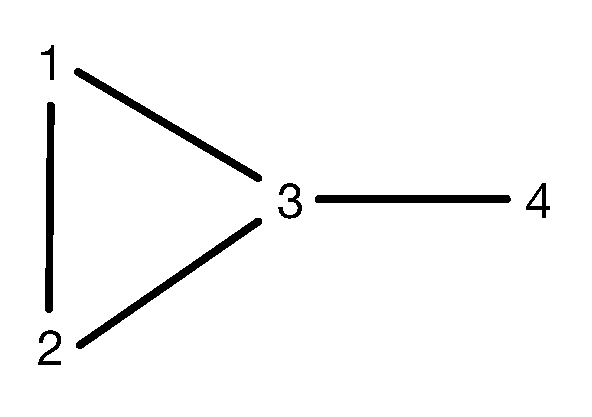
\includegraphics[scale=.5]{../figures/final-graph.pdf}
\end{center}
i.e. $G = (\{1,2,3,4\}, \{(1,2), (2,3), (3,1), (3,4)\})$.
\begin{enumerate}
\item List the bases and circuits of the graphic matroid $M_G = (E, I)$ for $G$.
\item Write down a list of inequalities describing the matroid polytope of $M_G$. \textbf{Hint: }\footnote{You should be able to get away with only 5 inequalities apart from the nonnegativity constraints, but it's ok if you write more.}
\item Let $I' = \{F \subset E:  d_F(3) \leq 2\}$. That is, $I'$ is the set of subgraphs of $G$ with at most $2$ edges incident to the vertex $3$. Write down a list of inequalities describing the polytope
$$ \conv(1_F: F \in I \cap I').$$
\end{enumerate}

\indent \textbf{Solution:}
\begin{enumerate}
\item The bases are all spanning trees, i.e.
$$\{(1,2),(2,3),(3,4)\}, \{(1,2),(1,3),(3,4)\}, \{(1,3), (2,3), (3,4)\}.$$
The circuits are all the cycles, which is just $\{(1,2), (2,3), (1,3)\}$.
\item The matroid polytope $P$ is $x \in \R^E$ such that $x_e \geq 0$ and $x(S) \leq r(S)$ for all $S \subset E$. Thus, apart from the nonnegativity constraints, we obtain $2^4 = 16$ inequalities; one for each subset of the edge set $E$. From considering the singleton sets $S$, we have the inequalities $x_e \leq 1$ for every $e \in E$. If $S$ is a forest, then we obtain the inequality $x(S) \leq |S|$, but these inequalities are implied by $x_e\leq 1$. Thus we are left to consider the two non-forests, which are $S = E$ and the triangle $S= \{(1,2), (2,3), (1,3)\}$. Again, the inequality from $E$ is implied by the inequality from the triangle, which is $x_{(1,2)} + x_{(2,3)} + x_{(3,1)} \leq 2$. Thus the final description is
$$ P = \{x: 0 \leq x_e \leq 1, x_{(1,2)} + x_{(2,3)} + x_{(3,1)} \leq 2.\}$$
\item $I'$ is the independent sets of a partition matroid $M'$ where one of the parts is the edges incident to the vertex $3$ and is allowed to contain $2$ elements. The polytope $Q$ we are interested in is the matroid intersection polytope. The matroid intersection polytope is simply the intersection of the two matroid polytopes, so we just need to figure out the matroid polytope $P'$ for $M'$. We can proceed similarly as in part (a); this time we find that $P'$ is
$$ P' = \{x: 0 \leq x_e \leq 1, x_{(3,1)} + x_{(2,3)} + x_{(3,4)} \leq 2\}.$$
Thus the final polytope is
$$ Q = \{x: 0 \leq x_e \leq 1, x_{(3,1)} + x_{(2,3)} + x_{(3,4)} \leq 2,\; x_{(1,2)} + x_{(2,3)} + x_{(3,1)} \leq 2\}.$$
\end{enumerate}



\end{enumerate}




\end{document}
